%%%%%%%%%%%%%%%%%%%%%%%%%%%%%%%%%%%%%%%%%%%%%%%%%%%%%%%%%%%%%%%%%%%%%%
%	Source code for Stevan Dupor (smdupor@ncsu.edu) Submission for:
%	ECE592 Fall 2021
%	Homework 2
%
%	Compiled on Windows using TeXworks with pdfLaTeX+MakeIndex+BibTex
%
%%%%%%%%%%%%%%%%%%%%%%%%%%%%%%%%%%%%%%%%%%%%%%%%%%%%%%%%%%%%%%%%%%%%%%
%
%								LATEX CODE RESOURCES:
%
 %  [1]	Document initialization template source: divisbyzero.com
%
% [2]	Embedded MATLAB Code formatting adapted from public github gist source: https://gist.github.com/eyliu/120689
%
%%%%%%%%%%%%%%%%%%%%%%%%%%%%%%%%%%%%%%%%%%%%%%%%%%%%%%%%%%%%%%%%%%%%%%

%%%%%%%%%%%%%%%%%%%%%%%%%% [1]
\documentclass[12pt,portrait]{article}
%\usepackage{amssymb,amsmath,amsthm,amsfonts}
\usepackage{amsmath}
\DeclareMathOperator*{\argmin}{\arg\!\min}
\usepackage{multicol,multirow}
\usepackage{calc}
\usepackage{ifthen}
\usepackage[portrait]{geometry}
\usepackage[colorlinks=true,citecolor=blue,linkcolor=blue]{hyperref}
\usepackage{enumitem}
%\usepackage{xcolor}
\usepackage{graphicx}
\usepackage{listings}
\usepackage{color} 
%\usepackage[bitstream-charter]{mathdesign}
\usepackage{arev}
\usepackage[T1]{fontenc}

\usepackage{array}
\newcolumntype{P}[1]{>{\centering\arraybackslash}p{#1}}

\usepackage{datetime}
\yyyymmdddate
\newcommand\tab[1][1cm]{\hspace*{#1}}



\ifthenelse{\lengthtest { \paperwidth = 8.5in}}
    { \geometry{top=.5in,left=.5in,right=.5in,bottom=.5in} }
	{\ifthenelse{ \lengthtest{ \paperwidth = 297mm}}
		{\geometry{top=1cm,left=1cm,right=1cm,bottom=1cm} }
		{\geometry{top=1cm,left=1cm,right=1cm,bottom=1cm} }
	}
\pagestyle{empty}
\makeatletter
\renewcommand{\section}{\@startsection{section}{1}{0mm}%
                                {-1ex plus -.5ex minus -.2ex}%
                                {0.5ex plus .2ex}%x
                                {\normalfont\large\bfseries}}
\renewcommand{\subsection}{\@startsection{subsection}{2}{0mm}%
                                {-1explus -.5ex minus -.2ex}%
                                {0.5ex plus .2ex}%
                                {\normalfont\normalsize\bfseries}}
\renewcommand{\subsubsection}{\@startsection{subsubsection}{3}{0mm}%
                                {-1ex plus -.5ex minus -.2ex}%
                                {1ex plus .2ex}%
                                {\normalfont\small\bfseries}}
\makeatother
\setcounter{secnumdepth}{0}
\setlength{\parindent}{5pt}
\setlength{\parskip}{0pt plus 0.5ex}

\setenumerate[0]{label=(\alph*)}

% Define Matlab colors
\definecolor{MyDarkGreen}{rgb}{0.0,0.4,0.0}
\definecolor{MyPurple}{rgb}{0.3,0,0.4}
\lstloadlanguages{Matlab}
\lstset{language=Matlab, 
        frame=single,            
        basicstyle=\small\ttfamily,
        keywordstyle=[1]\color{blue}\bfseries,        % Define formatting of matlab functions
        keywordstyle=[2]\color{MyPurple},         % Define formatting for matlab arguments
        keywordstyle=[3]\color{blue}\underbar,  % Define formatting for user functions
        identifierstyle=,                     			  % Define formatless identifier
                                                % Define formatting for matlab comments
        commentstyle=\usefont{T1}{pcr}{m}{sl}\color{MyDarkGreen}\small,
        stringstyle=\color{MyPurple},             % Define formatting for matlab strings
        showstringspaces=false,                 
        tabsize=5,                              % Set indentstyle for matlab
        							  %	 Include matlab functions not part of the default set
        morekeywords={xlim,ylim,var,alpha,factorial,poissrnd,normpdf,normcdf},
        							% Define matlab function parameters
        morekeywords=[2]{on, off, interp},
								% Set of user functions
        morekeywords=[3]{},
        morecomment=[l][\color{blue}]{...},     % Set formatting for line continuation operator
        numbers=left,                           % Enable line numbering
        firstnumber=1,                          % Initialize line numbers
        numberstyle=\tiny\color{blue},          % Format line numbers
        stepnumber=5                            % Set increment size for line numbers
        }
%%%%%%%%%%%%%%%%%%%%%%%%%%%%%%%%%%%%%%%%%%%% DOCUMENT BEGINS -----------------------------------------------------------------------

\title{ECE563 Project 2- Stevan Dupor - smdupor@ncsu.edu - id: 000211897}

\begin{document}

%\raggedright
\footnotesize
\vspace{5cm}
\begin{center}
{\large
\textbf{NC State University\\
\vspace{1cm}
Department of Electrical and Computer Engineering\\
\vspace{1cm}
ECE 463/563: Fall 2021 (Rotenberg)\\
\vspace{1cm}
Project \#3: Dynamic Instruction Scheduling}\\}
\vspace{3cm}
by\\
\vspace{1cm}
{\huge STEVAN DUPOR}\\ 

\vspace{4cm}
\noindent\fbox{%
    \parbox{\textwidth}{%
NCSU Honor Pledge: "I have neither given nor received unauthorized aid on this project."\\
Student’s electronic signature:  \underline{     Stevan M Dupor        }\\
Course Number: \underline{        563       }}}
\pagebreak
\end{center}

\section{Introduction and Methods}
This project involved implementing a valueless simulator for a superscalar out of order (OOO) processor. The simulator permits arbitrary-fixed-width execution throughout the pipeline, and simulates the movements of instructions from an instruction trace through said pipeline. As mentioned, the simulator is valueless, so no actual instructions are loaded -- the intent is to study the effects of parameters like Reorder buffer (ROB) and issue queue (IQ) size on Instruction Per Cycle (IPC) as the permitted width is changed. Further simplifications include perfect branch prediction, and perfect cache performance such that no instructions need be squashed to handle a mispredicted branch, and all stalls result from head-of-line blocking in the pipeline, be this due to Read-after-write (RAW) hazards or true dependencies, limitations on the ROB/IQ size, or limitations on the pipeline width. 
 
The simulator is implemented in C++ (2011 standard), and is implemented completely procedurally. Loading of traces into memory is abstracted from the pipeline simulation, and performed in a complete discrete step. Each phase of the pipeline is simulated by a section of a master function, and pipeline registers are simulated by STL vectors which hold pointers to instructions that are emplaced within these registers at any given time. The ROB and IQ are implemented as fixed-size circular arrays. 

Numerous experiments across varying width, ROB size, and IQ size parameters were conducted across multiple traces, and plots of these results as well as discussion of the findings follow in proceeding sections. The experiment configuration/automation and data collection via comma-separated-value file were performed using C++ (code excluded from submission for convenience). The data analysis and plots were implemented in Python -- code also excluded from submission for convenience.

\section{Experiment A: Fixed, Large ROB, varying Width and IQ size}
The first series of experiments were concerned with analysis of of a fixed-size ROB of 512 entries to eliminate the possiblity of full-ROB stalls. For each available trace (GCC and Perl), the IQ size was swept from 8 to 256 entries, across 1, 2, 4, and 8-wide superscalar pipelines. The results of these experiments, in the form of IPC curves, are displayed in plots below.

\subsection{Figures of GCC and Perl Trace IPC w/ Varying IQ}
The results of the GCC trace with varying IQ are displayed in Figure ~\ref{fig:plot1}, and those for the Perl trace in Figure ~\ref{fig:plot2}.
\begin{figure}[h!]
\centering
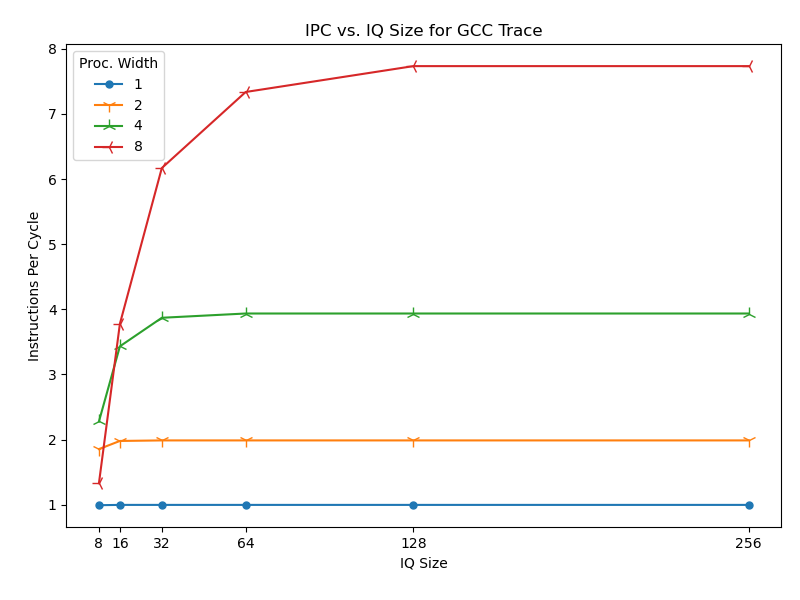
\includegraphics[width=5in]{iqs_gcc.png}
\caption{GCC trace, Varying IQ size}
\label{fig:plot1}
\end{figure}

\begin{figure}[h!]
\centering
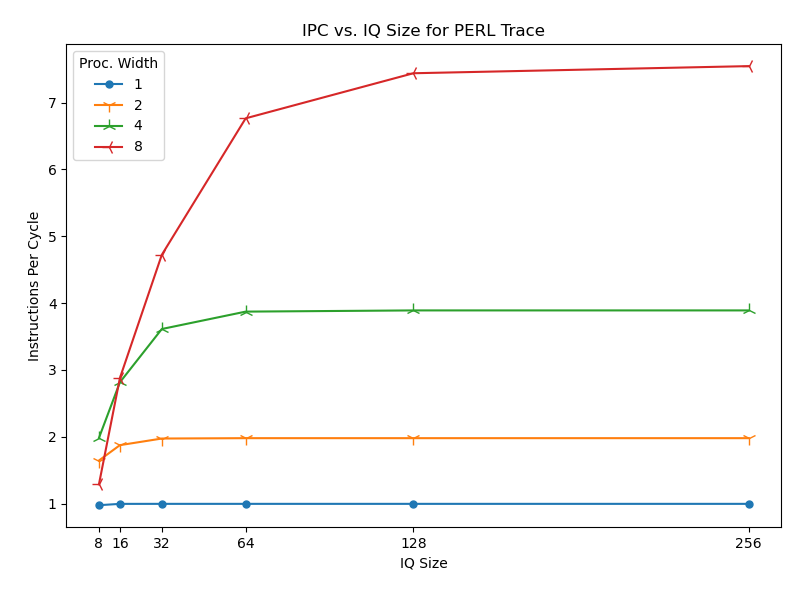
\includegraphics[width=5in]{iqs_perl.png}
\caption{Perl trace, Varying IQ size}
\label{fig:plot2}
\end{figure}

\subsection{Discussion of GCC and Perl Trace IPC w/ Varying IQ}
Notably, for both of these plots, all Instruction per Cycle curves approach an asymptote of approximately the \textbf{Width} of the curve in question. This is a logical limit on performance -- with zero stalls in execution, we can expect to only ever execute WIDTH instructions simultaneously as there are no other processing units besides the maximum contained in WIDTH. 

As a further point, I find that these curves quickly (exponentially) approach this asymptote, but the "room" for growth is much shorter as the width is smaller. In other words, a processor of WIDTH = 1 is already approximately at the asymptote at an IQ of 8, a processor of WIDTH = 2 at IQ=16, and so on. The logic that drives this trend is also fairly easy to derive -- since the ROB will not bottleneck, and the only bottlenecks in the system are the WIDTH of the frontend stages and the size of the IQ: \textbf{when the width of the frontend stage is a more serious bottleneck than the size of the IQ, increasing the size of the IQ will not lead to higher performance}. In other words, instructions can only come into the IQ one per cycle at WIDTH=1, which leads to limited opportunities for bottlenecks to form in an IQ that is 8 or 16 times the size of the WIDTH. Further analysis of the benchmark traces is likely to reveal that the main drivers of this bottleneck are large "gluts" of multi-cycle instructions, which are significantly more rare (especially for 5 cycle/instruction length instructions) than single-cycle instructions. So, instructions which would be stuck in the IQ waiting for data from long multi-cycle instructions in the execute stage trends towards not bottlenecking as IQ grows beyond these critical points. The numeric results of these critical points are reviewed in Table ~\ref{tab:tab1}.

A further point of discussion is the difference between these two plots for the same configuration (and differences between the critical points in the table). It is visually observable that the GCC trace benefits more from early growth in the IQ size, which means that at small sizes, for the GCC trace as compared to Perl, the IQ is the more serious bottleneck as compared to the Perl trace. Also, I note that the overall asymptotic performance of the GCC trace is slightly better than the Perl trace. I believe these points imply that the \textbf{GCC trace has more true dependencies between instructions, which means it benefits more from a larger IQ} (as the full pipeline need not stall while instructions wait for data to become ready in the ROB). However, regarding the second point about aysmptotic best-cases: I believe that the \textbf{Perl trace may contain statistically more multi-cycle instructions}, which cannot be forced to execute faster even with larger IQ/ROB buffer sizes.

In fact, upon running a simple instruction length count of the simulated traces, I am able to \textbf{confirm my prior claim that the Perl trace contains more slow 5-cycle instructions} than the GCC trace. The GCC trace contains 70.49 \% single-cycle instructions, 10.2\% 2-cycle instructions, and 19.29\% 5-cycle instructions. Conversely, the Perl trace contains 65.86\% single-cycle instructions, 9.21 \% 2-cycle instructions, and 24.93\% 5-cycle instructions. From this, it is clear that the tradeoff in the Perl trace is an increase of 5.64\% in 5-cycle instructions as compared to GCC, with the shorter/faster instructions being inversely reduced. 

%%%%%%%%%%%%%%%%%%%%%%%%%%%%%%%%%%%%%%%% REVISIT PERL AND GCC %%%%%%%%%%%%%%%%%%%%%%%%%%%%%%

\begin{table}[h]
%\tiny
\centering
\begin{tabular}{|P{2cm}|P{5cm}|P{5cm}|}
\hline
Width &  GCC Benchmark {\tiny $\argmin(IQ_{size}) = \{IPC_{width} \geq 0.95 \cdot IPC_{best}\}$ }&  Perl Benchmark {\tiny $\argmin(IQ_{size}) = \{IPC_{width} \geq 0.95 \cdot IPC_{best}\}$ }\\
\hline
Width=1 & 8 & 8 \\
Width=2 & 16 & 32 \\
Width=4 & 32 & 64 \\
Width=8 & 64\textcolor{MyDarkGreen}{$^{^{1}}$} & 128 \\
\hline
\end{tabular}
\caption{ \small Optimized IQ\_SIZE per WIDTH: The minimum IQ\_Size that still achieves within 5\% of the IPC of the largest IQ\_SIZE\\{\tiny \textcolor{MyDarkGreen}{(1): The GCC Width=8 value of 64 was chosen because this value was within $\frac{2}{5}$s of one percent of the 5\% cutoff, eg $p \leq 5.1357$\%, which is quite close to the whole-number threshold. This choice is especially attractive when considered in the light of die area and cost.}}}
\label{tab:tab1}
\end{table}


\section{Experiment B: Fixed IQ, varying Width and ROB size}
The second series of experiments were concerned with exploring the effects of the ROB size across different widths, for the same two traces. Notably, the "ideal" issue queue sizes from Table ~\ref{tab:tab1} were used for each Width, and the ROB sizes were swept from 32 to 512 entries in powers of two.

\subsection{Plots of IPC for ROB Size Experiments}
The plotted results from each of these traces are displayed in Figures ~\ref{fig:plot3} and ~\ref{fig:plot4}, below.

\begin{figure}[h!]
\centering
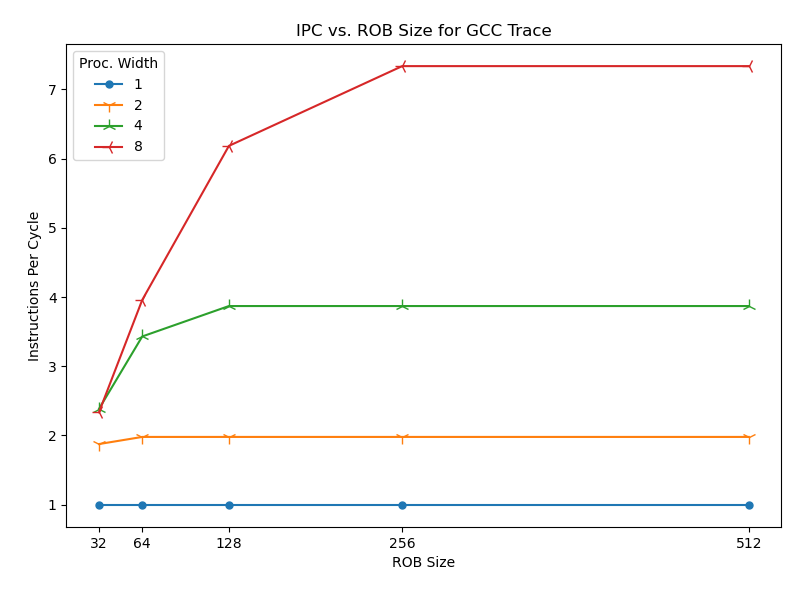
\includegraphics[width=5in]{rob_gcc.png}
\caption{GCC trace, Varying ROB size}
\label{fig:plot3}
\end{figure}

\begin{figure}[h!]
\centering
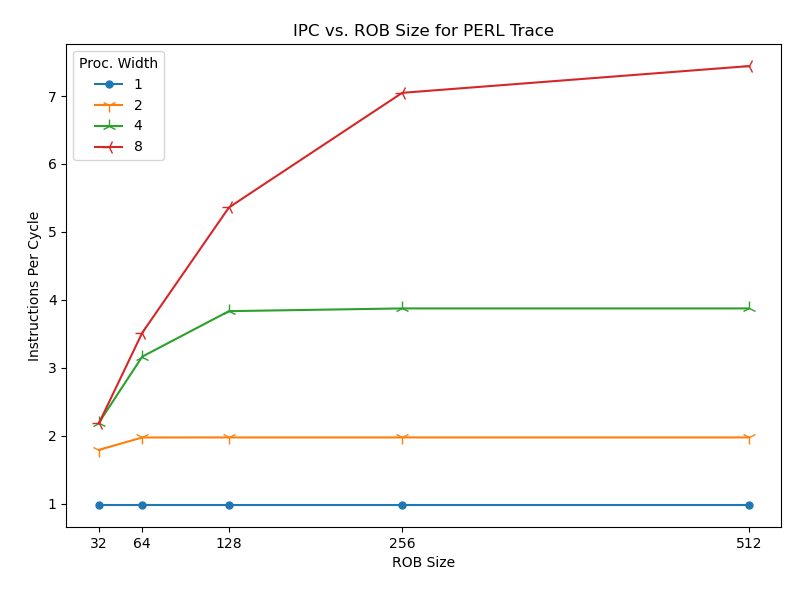
\includegraphics[width=5in]{rob_perl.png}
\caption{Perl trace, Varying IQ size}
\label{fig:plot4}
\end{figure}

\subsection{Discussion of ROB Size Experiments}
In this series of experiments, I observe similar expected asymptotic trends; however, I note that the growth rate of IPC in the exponential sections is less than observed in the IQ experiments. In particular, the growth in the Perl trace is slower, which lends greater weight to the claim made in the prior discussion section that the Perl trace likely contains more multi-cycle instructions: These are more likely to stall at the ROB because this is the point in the pipeline where long-execute instructions will tend to "pile up."

\section{Conclusions and Roadmap}
The implementation of the simulator and experiments were an excellent opportunity to reinforce the concepts of the scalar OOO pipeline, and the requirement of various bypasses to avoid deadlocks in the simulation. A natural roadmap progression for this project is to implement the support of several simplified or omitted features, namely: Imperfect caches with long cycle stalls, Imperfect branch prediction requiring in-pipeline instructions to be squashed, and fully-featured instructions with values. With these extensions, this simulator could perform more like an emulator, and many more parameters be studied by gathering execution statistics within the C++ code.

%\begin{enumerate}
%\item
%Bracketing search was performed, and the found range was determined to be (0.8, -0.25) to (-0.3714, -0.5103). See code for details.
%\item
%Golden section search was performed. Iterations and interim datapoints outlined in below table; see code for details.
%\begin{table}[h]
%%\tiny
%\begin{tabular}{|r|c|c|c|c|c|}
%\hline
%Iteration $k$&$a_k$&$b_k$&$f(a_k)$&$f(b_k)$&New Uncertainity Level\\
%\hline
%1 &(0.3526, -0.3494)&(0.5235, -0.3115) &0.1232&0.2080&[0.1709, 0.0380]\\
%2 &(0.2469, -0.3729)&(0.3526, -0.3494)&0.1080 & 0.1232&[0.1056, 0.0235]\\
%3 &(0.1816, -0.3874)&(0.2469, -0.3729)&0.1127&0.1080&[0.0653, 0.0145]\\
%4 &(0.2469, -0.3729)&(0.2873, -0.3639)&0.1080&0.1104&[0.0403, 0.0090]\\
%5 &(0.2220, -0.3784)&(0.2469, -0.3729)&0.1085&0.1080&[0.0249, 0.0055]\\
%6 &(0.2469, -0.3729)&(0.2623, -0.3695)&0.1080&0.1084&[0.0154, 0.0034]\\
%7 &(0.2374, -0.3750)&(0.2469, -0.3729)&0.1080&0.1080&[0.0095, 0.0021]\\
%\hline
%\end{tabular}
%\end{table}

%\item
%$R = 1001$
%\end{enumerate}
%\pagebreak
%
%
%
%\section{P6}
%\begin{figure}[h]
%\centering
%\includegraphics[width=5in]{p6a.PNG}
%%\caption{\textcolor{red}{Wireshark screencap for Question 1-4. Notations in RED.}}
%\end{figure}


%\textcolor{blue}{ Fraction of BW Filled With Headers = $\displaystyle \frac{nh}{nh+M}$}

%\textcolor{blue}{The probability of event $X_k$ with k active users is $\displaystyle P(X_k=n) = {30 \choose n}0.2^n \cdot (0.8)^{(30-n)}$ \\ The average number of active users is $30 %\cdot (0.2) =$ 6 users.\\ The probability of an overloaded link (k > 15) is $\displaystyle \sum_{n=16}^{30} {30 \choose n}0.2^n \cdot (0.8)^{(30-n)}$  }


%\begin{figure}[h]
%\includegraphics[width=7in]{problem7-ping-plot.png}
%\caption{\textcolor{blue}{One-way transit time from Raleigh, NC, USA as a function of distance in km}}
%\begin{center}
%	\hyperlink{code_problem_7}{Link to MATLAB Code}\\
%	\hyperlink{ping_figures_problem_7}{Link to Figures of ping command output}
%\end{center}
%\end{figure}



%\begin{figure}[h]
%\centering
%\includegraphics[width=5in]{tracert_vu_nl.png}
%\caption{\textcolor{blue}{Traceroute from Raleigh, NC, to Amsterdam, NL (Vrije Universiteit): vu.nl}}
%\end{figure}
%
%\pagebreak
%\hypertarget{code_p_26}{}
%\hyperlink{p_26}{LINK TO: Question and Answer for Problem 26}
%\section{Appendix A: MATLAB Code For Problem 26}
%\lstinputlisting{p26.m}

\end {document}